\documentclass[10pt]{article}
\usepackage[polish]{babel}
\usepackage[utf8]{inputenc}
\usepackage[T1]{fontenc}
\usepackage{graphicx}
\usepackage[export]{adjustbox}
\graphicspath{ {./images/} }
\usepackage{amsmath}
\usepackage{amsfonts}
\usepackage{amssymb}
\usepackage[version=4]{mhchem}
\usepackage{stmaryrd}

\title{LIGA MATEMATYCZNA \\
 im. Zdzisława Matuskiego \\
 PAŹDZIERNIK 2017 \\
 SZKOŁA PODSTAWOWA }

\author{}
\date{}


\begin{document}
\maketitle
\section*{ZADANIE 1.}
Czy liczbę 7777777 można przedstawić jako sumę dwóch liczb pierwszych?

\section*{ZADANIE 2.}
Oblicz pole figury przedstawionej na rysunku, gdzie odpowiednie kąty są proste.\\
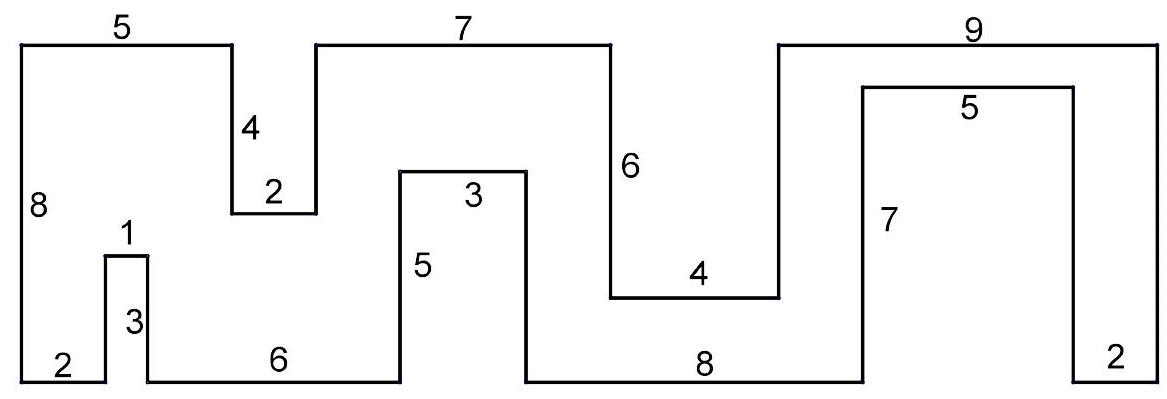
\includegraphics[max width=\textwidth, center]{2024_11_21_a5b230033f508f480714g-1(1)}

\section*{ZADANIE 3.}
Pan Adam jest staruszkiem, ale nie ma jeszcze stu lat. Dla treningu lubi układać i rozwiązywać łamigłówki liczbowe. Właśnie zauważył, że w ubiegłym roku jego wiek był liczbą całkowitą podzielną przez 8, a w przyszłym roku będzie liczbą podzielną przez 7. Ile lat ma pan Adam obecnie?

\section*{ZADANIE 4.}
Liczbą palindromiczną nazywamy liczbę, która czytana od lewej do prawej oraz od prawej do lewej jest taka sama. Ile jest liczb palindromicznych trzycyfrowych podzielnych przez 4?

\section*{ZADANIE 5.}
Wewnątrz pięciokąta foremnego \(A B C D E\) obrano punkt \(F\) w taki sposób, że trójkąt \(A B F\) jest równoboczny. Oblicz miarę kąta \(C F E\).\\
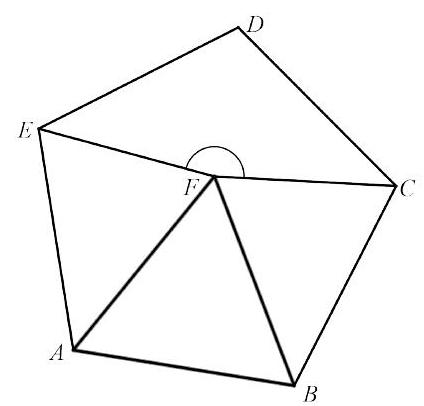
\includegraphics[max width=\textwidth, center]{2024_11_21_a5b230033f508f480714g-1}


\end{document}